% This LaTeX was auto-generated from MATLAB code.
% To make changes, update the MATLAB code and export to LaTeX again.

\documentclass{article}

\usepackage[utf8]{inputenc}
\usepackage[T1]{fontenc}
\usepackage{lmodern}
\usepackage{graphicx}
\usepackage{color}
\usepackage{hyperref}
\usepackage{amsmath}
\usepackage{amsfonts}
\usepackage{epstopdf}
\usepackage[table]{xcolor}
\usepackage{matlab}

\sloppy
\epstopdfsetup{outdir=./}
\graphicspath{ {./example9_1_images/} }

\begin{document}

\matlabtitle{EM Algorithm example (Example 9.1)}

\begin{par}
\begin{flushleft}
Start defining the data set:
\end{flushleft}
\end{par}

\begin{matlabcode}
D = [3,3;
    4,10;
    9,6;
    14,8;
    18,11;
    21,7];

centers = [3,3;
           4,10];

[p1,c1] = E_step(D, centers)
\end{matlabcode}
\begin{matlaboutput}
p1 = 2x6    
    1.0000         0    0.4767    0.4160    0.4053    0.4671
         0    1.0000    0.5233    0.5840    0.5947    0.5329

c1 = 1x6    
     1     2     2     2     2     2

\end{matlaboutput}
\begin{matlabcode}
centers_2 = M_step(D, p1)
\end{matlabcode}
\begin{matlaboutput}
centers_2 = 2x2    
    8.4178    5.0946
   10.4632    8.9897

\end{matlaboutput}
\begin{matlabcode}

[result, probs, cl] = em_algorithm(D, centers, 0.5)
\end{matlabcode}
\begin{matlaboutput}
result = 2x2    
    6.3427    6.2224
   16.6020    8.6542

probs = 2x6    
    0.9096    0.8905    0.9012    0.1043    0.0449    0.0930
    0.0904    0.1095    0.0988    0.8957    0.9551    0.9070

cl = 1x6    
     1     1     1     2     2     2

\end{matlaboutput}
\begin{matlabcode}

D(:,3) = cl;
c1 = D(:,3) == 1;
c2 = D(:,3) == 2;

scatter(D(c1,1),D(c1,2), 'MarkerFaceColor', 'b');
hold on
scatter(result(1,1),result(1,2), 'MarkerFaceColor', 'b');
scatter(D(c2,1),D(c2,2), 'MarkerFaceColor', 'g');
scatter(result(2,1),result(2,2), 'MarkerFaceColor', 'g');
hold off
\end{matlabcode}
\begin{center}
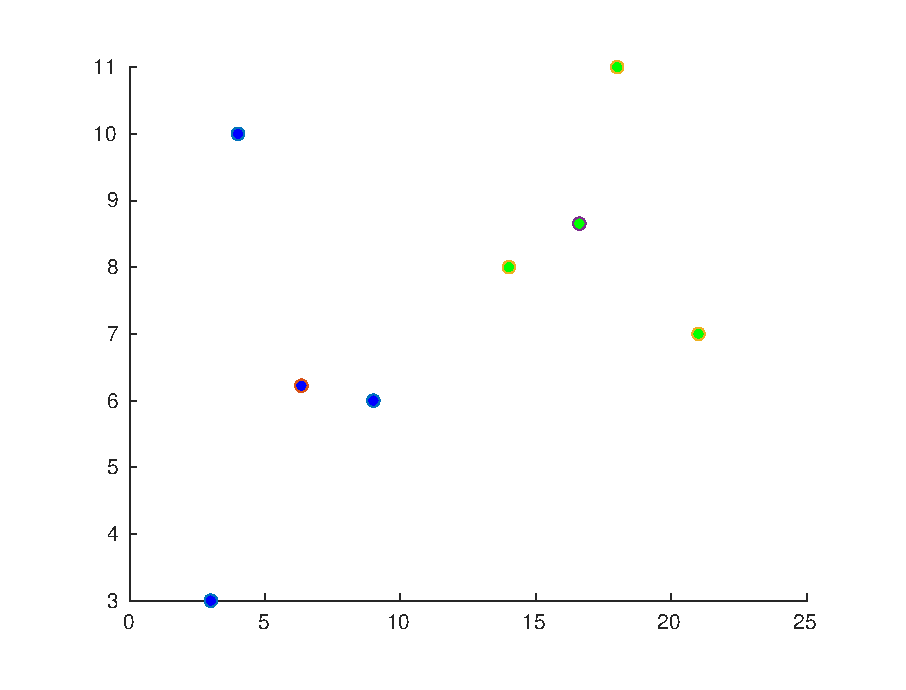
\includegraphics[width=\maxwidth{56.69844455594581em}]{figure_0.eps}
\end{center}
\begin{matlabcode}

\end{matlabcode}


\begin{matlabcode}
function d = distance(X, Y, m)
    n = length(X);
    d = 0;
    for i=1:n
        d = d + abs(X(i)-Y(i))^m;
    end
    d = sqrt(d);
end

function sse = SSE(probs, data, centers, p)
    sse = 0;
    for i = 1:length(centers)
        for j = 1:length(data)
        sse = sse + probs(i,j)^p*distance(data(j,:),centers(i,:),p)^2;
        end
    end
end

function [probs,clusters] = E_step(data, centers)
    k = length(centers);
    n = length(data);
    distances = zeros([k,n]);
    for i = 1:k
        for j = 1:n
            distances(i,j) = distance(data(j,:),centers(i,:),2)^2;
        end
    end

    full_dists = sum(distances,1);
    probs = (full_dists - distances )./ full_dists;

    [c,idx] = min(distances,[],1);
    clusters = idx;
end

function new_centers = M_step(data,probs)
    sq_probs = probs.^2;
    sum_sq_probs = sum(sq_probs,2);
    new_centers = sq_probs * data;
    new_centers = new_centers ./ sum_sq_probs;
end

function [centers, probs, clusters] = em_algorithm(data, in_centers, eps)
    dif = inf;
    while dif > eps
        [probs,clusters] = E_step(data, in_centers);
        centers = M_step(data, probs);
        dif = sum(centers - in_centers);
        in_centers = centers;
    end
    [probs,clusters] = E_step(data, centers);
end
\end{matlabcode}

\end{document}
